\documentclass[10pt,letterpaper]{article}
\usepackage{hyperref}
\usepackage{cogsci}
\usepackage[nodoi]{apacite}
\usepackage{pslatex}
\usepackage{pdfsync}
\usepackage{amsmath}
\usepackage{graphicx}
\usepackage{topcapt}
\usepackage{color}
\usepackage[english]{babel}
\usepackage{array}
\usepackage{pbox}
\usepackage[usenames,dvipsnames]{xcolor}
\usepackage[section]{placeins}


\title{Large-scale investigations of variability in children's first words}
\author{{\large \bf Rose M. Schneider} \\ \texttt{rschneid@stanford.edu}\\ Department of Psychology \\ Stanford University \\ 
\And {\large \bf Daniel Yurovsky} \\ \texttt{yurovsky@stanford.edu} \\ Department of Psychology \\ Stanford University \\ 
\And {\large \bf Michael C. Frank} \\ \texttt{mcfrank@stanford.edu} \\ Department of Psychology \\ Stanford University \\ }

\begin{document}
\maketitle


%ABSTRACT
\begin{abstract}
A child's first word is an important step towards language. Aggregated across children, the distribution of these first productive uses of language can act as a window into early cognitive and linguistic development. We investigate both the variability and predictability in children's first words across four new datasets. We find, first, that children's first words tend to emerge earlier than previously estimated: more than 75 percent of children produce their first word before their first birthday. Second, we find a high degree of consistency in the types of things children name in their first words, independent of the age at which they are produced. Finally, we show that the particular words that children produce first are predictable from two linguistic factors: input frequency and phonological complexity. Together, our results suggest a degree of independence between early conceptual and linguistic development.

\textbf{Keywords:}
Language acquisition, word learning, cognitive development
\end{abstract}

%%INTRODUCTION%%%%
\section{Introduction}

Over the course of their first years, children rapidly go from speechless infants to toddlers producing and learning language at an astounding rate \cite{fenson1994}. Marking the beginning of productive verbal language, a child's first word is an important and measurable insight into what a child is willing and able to talk about at that point in their development. Yet, in contrast to later behaviors, children's first words often emerge during intimate moments between children and caregivers that are difficult for external observers to record or measure. Here we leverage large-scale data from parental reports to ask what children's first words reveal about two key issues in early language learning: the time-course of the emergence of language, and the relation between conceptual and linguistic development. In three sets of analyses, we explore when a first word is likely to emerge, as well as the distribution of conceptual categories of these first words in both early and later speakers. Finally, we turn to the factors that predict which words are more likely to be a child's first.

Infants begin to show an aptitude for language from a very early point in development. For instance, 1-month-old infants already prefer to listen to child-directed speech over adult-directed speech \cite{cooper1990}. Over the course of the first year, infants are learning to recognize and segment the distinctive sounds and word forms of their native language \cite{kuhl2004,werker2005}. Additionally, by 6--9 months, many infants already show a tendency to look to named targets when they hear common nouns, suggesting early beginnings for form-meaning mapping as well \cite{tincoff2012,bergelson2012}. Infants' abilities to comprehend language thus appear to be reasonably well-developed prior to 12 months. Additionally, as early as 12 weeks, children also begin producing the sounds of their native language in babble, suggesting an early beginning to language production \cite{kuhl2004}. However, developmental norms suggest that the typical child will produce their first word at 12 months. Is this early lag between comprehension and production real, or only apparent?

What is the relationship between children's linguistic and conceptual development? Typically-developing monolingual children show correlations between some cognitive achievements and their language production; for example, acquisition of words about disappearance is correlated with comprehension of object permanence \cite{gopnik1986}. But at a larger scale, conceptual development appears to play a more limited role: 2--5-year-old international adoptees learning English for the first time show the same gross patterns of development in vocabulary composition as monolingual infants. \cite{snedeker2007}. There are also striking convergences in early words across very different cultural contexts \cite{tardif2007}. Do patterns of first word productions---and their distribution across semantic categories---suggest any broader relationships between language acquisition and cognitive development? 

Because very early language is difficult to observe in the lab, in this study we leverage parent reports to learn about children's first words, and what they can reveal about the relationship between early conceptual and linguistic development. A child's first word is highly memorable for parents, and many parents record this milestone in baby books. We define a true ``first word'' as the consistent use of a form to communicate a particular meaning, whether or not that form matches the adult target form. While recognizing that parents may not share this definition, intuitively, we believe this is what parents tend to think they are reporting when they report first words, and found support for this across our datasets in parents reporting a first word as a phonological approximation of a more complex adult target.

Parent report has both substantial disadvantages and real advantages as a scientific measurement. One issue with any self-report measure is that there is no way to validate participants' responses. Another complication is that parents may be biased observers, and interpret word-like babble as productive communication. Additionally, the recollection of a first word may be subject to errors in memory recall, or other retrospective biases. Nevertheless, parent report is widely used as a measure of early child language, e.g. in the MacArthur-Bates Communicative Development Inventory (CDI), a vocabulary checklist that is both a reliable and valid measure of early vocabulary (\citeNP{fenson1994,fenson2007}, although the reliability of the earliest ages of the CDI has been questioned; \citeNP{feldman2000}). And in addition, self-reports are very easy to collect, making them ideal for large-scale investigations like the present study. 

To address some of the issues of bias in self-report, we gathered data from four sources. The first dataset was a survey filled out by parents who were members of a local children's museum. These parents were an ethnically diverse population with a higher education level than the general population and a demonstrated interest in their child's development, likely leading to a high level of engagement in their children's early language. Our second dataset was the Amazon Mechanical Turk parent population; this community is more diverse in terms of age, gender, education level, and socio-economic status (SES). Our third dataset came from parents in the psycholinguistic research community. We selected this population for its familiarity with the subject and because this community was most likely to have written records about first words. The data we received from all three of these surveys was generally very consistent, both within and across datasets, leading us to believe at the very least that any bias in one was likely in operation across all three. 

Our final dataset was drawn from \href{http://wordbank.stanford.edu}{Wordbank}, a large, open repository of CDI form data that aggregates across several samples including the updated CDI norming sample \cite{fenson2007}. This dataset was chosen because the CDI form asks a parent to report their child's  current productive vocabulary, and thus is free from any retrospective reporting biases that may skew our other surveys. Because the CDI contains a fixed set of words, it constrains the space of possible first words but also facilitates comparative analyses by reducing the space to a small, representative set.

Drawing on these datsets, we investigate the time-course of the emergence of productive language and potential factors that might lead to individual differences in linguistic development. First, we analyze variability in the age of first word onset, finding that 75\% of children are reported as producing a word prior to 12 months. Second, we ask whether the range of of first words varies with children's chronological age, allowing us to ask about the relationship between linguistic and conceptual development. This analysis yields no measurable differences, indicating that linguistic factors---rather than conceptual ones---likely constrain the set of first words. Finally, we show that two specific linguistic factors, input frequency and phonetic complexity, both predict the words that children are likely to say first.

%%GENERAL DATA METHODS%%
\section{General Methods}

Data for the study come from four datasets. Three of the four were surveys specifically designed for this study. 

%CDM
\subsection{Dataset 1: Museum Member Survey}

\subsubsection{Participants}

We sent out a very brief survey on children's first words to subscribed members of a large local children's museum. We received responses for 502 children (215 female, 285 male, and 2 with no reported sex; M age = 11 mo., median = 10 mo.). Several responses were translated into English where possible; one response could not be translated and was excluded from further analysis. 

\subsubsection{Method}

Parents completed a web-based survey. The survey asked parents to report their child's first word (excluding ``mama'' and ``dada''), the word referent, a description of the situation surrounding the first word, the child's age at time of utterance (10 mo. or younger, 11 mo., 12 mo., 13 mo., 14 mo.), the child's current age, and sex. Parents answered for only one child in this survey. We standardized responses and corrected obvious spelling errors. When the meaning of the word was not immediately apparent, we relied on the parent's description of the circumstances surrounding the word and/or the parent's classification of the word type.

\subsubsection{Exclusion of ``mama'' and ``dada''}

While many parents reported that their child's first word was ``mama'' or ``dada'' (or some equivalent or variant), we excluded these children from our analyses. First, parents may be motivated to hear these words very early in babble, even when the word is not being used in a meaningful or consistent way. Second, we were interested in the range of concepts represented in the words we analyzed. Therefore, we stressed in our surveys that parents were to report their children's first word \emph{other} than ``mama'' or ``dada'' to avoid this possibility and to detect a larger range of conceptual types. Additionaly in the MTurk dataset, we included a question asking whether the child's first word was ``mama'', ``dada,'' or another first word. In total, 1107/1650 (67\%) of children were reported to produce ``mama'' (N = 618) or ``dada'' (N = 489) first rather than another word (N = 543).

%SURVEY2
\subsection{Dataset 2: Amazon Mechanical Turk}

\subsubsection{Participants}

We recruited 1000 parents from Amazon Mechanical Turk (Mturk) to complete an in-depth survey on their children's first words. We restricted the survey to parents in the United States. This survey allowed parents to answer for multiple children. We received responses for 1671 children (813 female, 858 male; M age = 10 mo., median = 10 mo.). Responses from 21 children were excluded from subsequent analyses because they had not yet spoken (M age = 2.7 mo., median = 2 mo.). Responses in other languages were translated into English where possible; one response was excluded. After exclusions, this dataset contained responses from 996 parents and 1650 children's first words. Caregiver education levels were highly diverse (Elementary = 3; Some high school = 15; High school = 166; Some college = 309; College = 346; Some graduate school = 26; Graduate school = 131; N = 996).

\subsubsection{Method}

This survey was an extended version of the Museum survey, allowing for input for multiple children, and asking the respondent to list their highest level of education, child's birth order, sex, first word (excluding ``mama'' and ``dada''), word type, addressee of the first word, age at time of the word (0--24+ months), current age (0--18+ years), and both the languages of the first word and typically spoken at home.

Data were handled as in Dataset 1. Due to the larger sample size, more phonological and morphological variations appeared in parents' reports of children's productions. A final standardized form was selected, and the various original first word forms were recoded as that standardized form. For example, ``Dog dog,'' ``Doggy,'' ``Doggie,'' and ``Dogie'' were all coded as ``Dog.'' When necessary, we relied on the parent's description of the situation in this coding process.

%%%SURVEY 3
\subsection{Dataset 3: Psycholinguists }

\subsubsection{Participants}

We sent out a brief survey on children's first words to subscribed members of a Psycholinguistics listserv. We received 52 responses from this survey (26 female, 26 male; M age = 11.16 mo., median 11 mo.).

\subsubsection{Method}

Questions included on the survey were: The approximate phonological form of the first word, the age of utterance, when the parent recorded the word (if at all), the child's sex, the target word, the child's birth order (first or later born), and the child's current age. Data were handled similarly to Datasets 1 and 2. 

%%%%WORDBANK%%%%
\subsection{Dataset 4: Wordbank}

\subsubsection{Participants}

At the time of our analysis, the Wordbank database contained 8889 unique CDI Words and Gestures administrations. From these, we selected the 76 English-speaking children whose parents reported that they produced exactly one word (31 female, 45 male, M age = 10.63 mo., median = 11 mo.). Caregiver education levels were fairly diverse (Some high school = 4; High school = 24; Some college = 21; College = 17; Some graduate school = 1; Graduate school = 9). 

\subsubsection{Data preparation}

As responses were taken directly from the CDI, no data preparation was necessary.

%Analyses

\begin{table}[tb]
\centering
\begin{tabular}{cccc}
\hline
{\bf MTurk} & {\bf Museum} & {\bf Psycholinguists} & {\bf Wordbank} \\ 
\hline
\textbf{Dog} & \textbf{Ball} & Up & Baa Baa \\ 
No & \textbf{Hi} & More & Uh--Oh \\
\textbf{Ball} & \textbf{Dog}& \textbf{Hi} & Yum Yum \\ 
Bottle & Uh--Oh& \textbf{Cat} & \textbf{Woof Woof} \\ 
\textbf{Hi} & Duck  & \textbf{Bye} & \textbf{Hi} \\
\textbf{Bye} & Car &  & Vroom \\
Kitty & No &  & This \\
Baba & \textbf{Cat} &  & Meow \\
\textbf{Cat} & \textbf{Bye}&  & Bottle \\
Milk & Up, More &  & \textbf{Ball} \\
\hline 
\end{tabular}
\caption{\label{tab:top10} Top ten first words (excluding ``mama'' and ``dada'') from each of the four datasets we examined. Words repeated across more than 2 datasets are bolded. Included are only words with more than 1 instance.}
\vspace{-3em}
\end{table}

\section{Analyses}

Table \ref{tab:top10} shows the top ten words from each dataset. Overall, there is substantial consistency across the four datasets, with ``Hi'' appearing in all four, and ``Bye'', ``Ball'', ``Dog''/``Woof Woof'', and ``Cat'' appearing in three.

Below we report three primary analyses. Analysis 1 examines the age of first production, Analysis 2 describes the semantic categories of these words, and Analysis 3 predicts which words tend to be produced on the basis of phonological complexity and input frequency.

\subsection{Analysis 1: Age of First Word} 

Despite evidence for very early word comprehension \cite{tincoff2012,bergelson2012}, conventional wisdom holds that the first word emerges around 12 months. However, a child's first word is almost exclusively heard by a parent or other caretaker. Is this reported lag between comprehension and production real or apparent? 


%FIGURE 1
\begin{figure}[tb]
\center{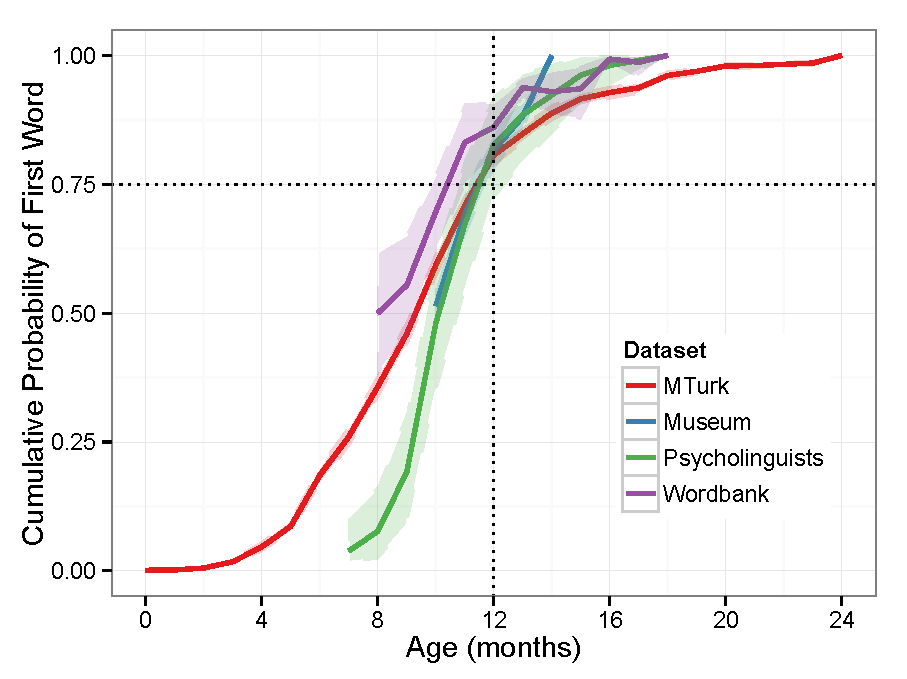
\includegraphics[width=.9\linewidth]{figures/Figure1.pdf}}
\caption{\label{fig:cdfs} Cumulative probability of a child having produced her first word across development. In all datasets, more than 75\% percent of children had produced their first word by their first birthday and more than half had produced their first word by 10 months. Shaded regions show 95\% confidence intervals computed by non-parametric bootstrap.}
\vspace{-1.4em}
\end{figure}

Using data from a total of 2,279 children we plotted the cumulative probability of a child having produced a first word as a function of their age and dataset (Figure~\ref{fig:cdfs}). Prior to 12 months, approximately 75\% of children had produced a first word, across all four datasets. This result was strikingly consistent across datasets, despite significant variance in the tails. 

Data from the Museum survey were truncated due to a ``ten months or earlier'' response option and showed the least age variability, with respondents modally choosing the earliest option. Data from Wordbank were also truncated due to the 8 month cutoff for the use of the CDI (as well as data sparsity in the oldest ages); nevertheless, Wordbank data showed the earliest word productions. One possibility is this may reflect a bias towards reporting at least one word, given the process of going through the entire CDI checklist; another possibility is that seeing the checklist allows parents to more thoroughly consider their child's early productions. 

Data from the MTurk survey showed a broader distribution of ages, perhaps due to the greater diversity (as well as larger size) of this sample. Some children were reported to be producing words implausibly early (e.g., 4 months). These responses are very likely (though not, to be fair, with absolute certainty) the result of reporting errors or biases. To estimate retrospective reporting biases, we regressed the mean age of first words against the time since the event in our largest dataset (MTurk, which had the most fine-grained age data), but did not find a significant relationship, suggesting no biases of this type that we could measure. On the other end of the spectrum, some respondents reported first words appearing after 18 months, a timeline which might raise clinical concerns. Indeed, in a population as large as this one, there are almost certainly some children with speech-language delays or other developmental disorders. Thus, this dataset is potentially valuable for estimating the right tail of the distribution in a diverse population. 

Finally, the Psycholinguist dataset shows a relatively later and steeper onset of word production than the other three (though it still reaches 75\% around 11 months). Given the high level of education of the respondents, it is likely that these children would have large early vocabularies \cite<e.g.>[et seq.]{hart1995}. On the other hand, the majority of these respondents recorded their child's first word at the time of production, decreasing concerns about retrospective report. Additionally, these respondents had training in psycholinguistics and were more likely to apply a more stringent standard (we shared our definition of a first word with respondents in the survey instructions). Thus we view the lack of very early respondents as prima facie evidence that first words before 9 months are rarer than our other surveys might lead us to believe.

In sum, we see some evidence for over-optimism (estimating first words earlier than we might expect) in a number of our datasets. It must be noted that, as our surveys were designed exclusively to ask about a child's first word, parents of later producers who had not spoken a first word yet may have been unwilling to take the survey, potentially skewing the age of production earlier. However, across the Museum, MTurk, and Psycholinguist datasets, more than 50% of the children were currently older than 2 years, meaning that later-producers are very likely included in these datasets. Additionally, we saw no evidence of retrospective reporting biases. A plausible account of this pattern is that first words---whether detected optimistically or realistically---are a memorable event whose date and context are recalled well. In addition, despite differences in the tails, there was a striking convergence between datasets in suggesting that most children in our sample produced a first word prior to their first birthday. 

\subsection{Analysis 2: Independence of Age and First Word}

The variability in children's age of first production gives us a natural tool for asking about the relationship between conceptual and linguistic development. All things being equal between age groups, younger children should be less conceptually sophisticated and hence might produce words for a more restricted range of concepts.\footnote{Of course, younger producers might be on average more conceptually sophisticated than older producers, but the current analysis assumes that other developmental factors (e.g. phonological development, language experience, etc.) also vary.} Alternatively, if the concepts that children most want to talk about are present early \cite{snedeker2007,snedeker2012,gleitman1990}, we should predict no difference in the distribution of first words for older and younger children. 

We ask here whether older children show a different distribution of first words.  We assigned words to the categories that appear on the CDI instrument (e.g., animals, games and routines, toys, people, etc.) and conducted our analysis over the category distribution of words (a loose proxy for their semantic distribution). We assigned CDI categories consistently across datasets for words that did not appear on the CDI word list. Ninety-one children were excluded because their first word could not be categorized. 

Figure~\ref{fig:cdi_cats} shows the frequencies of the CDI categories split by age (\textless{12 mo.}, \textgreater{12 mo.}) and grouped by dataset. Especially in the two larger datasets, the distribution across categories was virtually indistinguishable. Animals, Games and Routines, Toys, and People were all frequent first word categories, and all seemed equally compelling as a first word for both early and later producers. Data for later speakers in Wordbank was sparse, because children were selected for this analysis when they were producing exactly one word, according to parental report on the CDI, and only 27 children met this criterion.


%CDI cats
\begin{figure*}[t]
\begin{center}
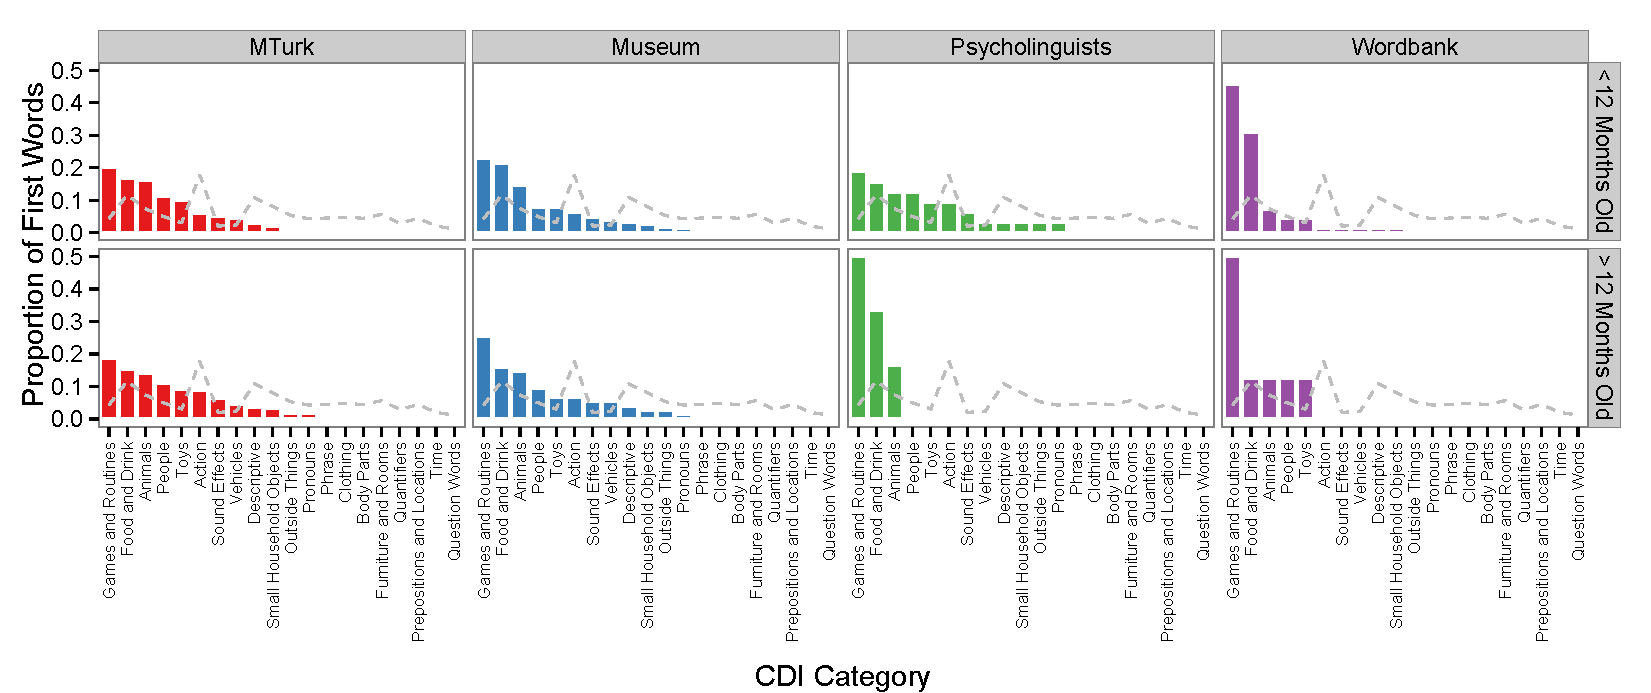
\includegraphics[width = .9\textwidth]{figures/Figure2.pdf}
\end{center}
\caption{Proportion of children's first words falling into each CDI category. The datasets showed a high degree of consistency, with most first words referring to animals or games and routines. These distributions were highly consistent between older and younger children, suggesting that first words are driven by linguistic rather than conceptual factors. The dashed line shows the baseline distribution of CDI categories.}
\label{fig:cdi_cats}
\vspace{-1em}
\end{figure*}


\begin{table}[tb]
\centering
\begin{tabular}{ccc}
\hline
Data Set & CDI Category & First Word \\ 
  \hline
  MTurk & (-0.23, 0.04) & (-0.31, 0.12) \\ 
  Museum & (-0.25, 0.25) & (-0.10, 0.50) \\ 
  Psycholinguists & (0.00, 1.33) & (0.00, 1.11) \\ 
  Wordbank & (-0.72, 0.83) & (-0.59, 0.69) \\ 
   \hline
\end{tabular}
\caption{\label{tab:ent_diffs} 95\% confidence intervals on differences in the entropy of First CDI Category and First Word between older and younger children.}
\vspace{-1em}
\end{table}

To quantify differences in variability across age, we asked whether the entropy of children's word or category distributions were different for our older and younger children \cite{shannon1948}. Differences in entropy would signal differences in the breadth of the distribution across words or categories. Because entropy is sensitive to sample size, for each dataset we split children into older and younger groups, and then down-sampled the larger group to the size of the smaller one. We then computed the difference in entropy for children in the older group as compared to the younger group at both the word and category level. For each dataset and for both words and CDI categories, we used non-parametric bootstrap resampling to identify whether the observed difference in entropy was significant at the $p = .05$ level. For all datasets and measures, the 95\% confidence interval for entropy differences included 0, indicating no significant difference in entropy across ages (Table\ref{tab:ent_diffs}).

In our exploration of the data, we found one word that was both highly frequent and potentially linked to conceptual development: ``no.'' Negation is a complex construct, and various functions of negation (denial, refusal, nonexistence) are posited to emerge at different points in a child's development \cite{pea1982}. We coded instances of ``no'' (in the MTurk data, where the majority of instances were reported) based on parent descriptions of the situation surrounding the first word. Of 108 children producing ``no'' as a first word, 40\% did so as a refusal; there were no instances of ``no'' being used as denial, which is acquired later \cite{pea1982}. 

In sum, despite producing a first word during different points in their conceptual development, both early and later producers in our sample chose to talk about the same semantic categories, and in many cases, the same things (see Table \ref{tab:top10}). This finding suggests that first words tend to reflect concepts that are available early. Why then do children consistently pick certain words to talk about? In the next analysis, we examine the role of input frequency and phonological complexity in determining which words are predicted. 

\subsection{Analysis 3: Predicting First Words}

% Our previous analyses found a high degree of consistency among children's first productions. Independent of their age, children seem to produce the same first words. Why these words? 
Our analyses, along with those of \citeA{snedeker2012} suggest a degree of independence between conceptual and linguistic development. Thus, we hypothesize that children's first words should be constrained by other factors. To say her first word, a child must minimally have been exposed to that word, and also be able to pronounce it. We ask whether children's first words are predicted by two factors known to predict the acquisition of words more broadly: input frequency, and phonetic complexity \cite{morgan1996,goodman2008}.
% Here we investigate the role of linguistic input and speech production ability.

% \subsubsection{Method}

% Each of our datasets consists of a set of words that children produced, and the number of children who produced each of these words. 
The goal of our analysis is to determine both why some first words were produced more frequently than others (e.g. ``dog'' vs. ``asleep''), and also why some words were never first words at all (e.g. ``animal''). Because the set of words that were never produced is infinite, we needed to constrain our set of candidate first words to a small, representative, finite set. For this reason, and to ensure fair comparison across datasets, we restricted our set of words to the 385 words that appear on the CDI Words and Gestures form. 
% We thus selected the subset of first words in each of our datasets that appeared on the CDI, and asked how many of our children produced each.


To estimate the approximate frequency with which children hear each of these words, we tabulated the number of times each appears in CHILDES (a large corpus of parent-child interactions;  \citeNP{macwhinney2000}). To ensure a representative sample, we counted the number of appearances of each word in a child's mother's speech across all of the corpora in the North American subset. These frequencies were then log-transformed.  To estimate phonetic complexity, we chose a simple, theory-independent measure: number of phonemes. For each of this same subset of words, we queried the MRC Psycholinguistic Database \cite{Wilson1988}. Number of phonemes is an imperfect measure of phonetic complexity---it misses differences in articulatory complexity that contribute to the relative difficulty of \emph{producing} different words (e.g. ``truck'' vs. ``bunny'')---but it does capture some of the variability among the CDI words.

To predict the number of observations of each of a set of a categorical outcomes, the standard statistical model is Poisson regression, but this method behaves poorly when distributions violate its assumptions through high variance (overdispersion) and too many zeros. To adjust for these violations, we used a hurdle model \cite{mullahy1986}. This model predicts the number of observed counts through a combination of two processes: a binomial threshold (hurdle) that first determines whether a count is zero or greater, and then a second component which determines the size of the count if it is non-zero. Because the datasets were of such different sizes, we fit a separate hurdle model to each and examined consistency in the estimated parameters across datasets.

\begin{figure}[tb]
\center{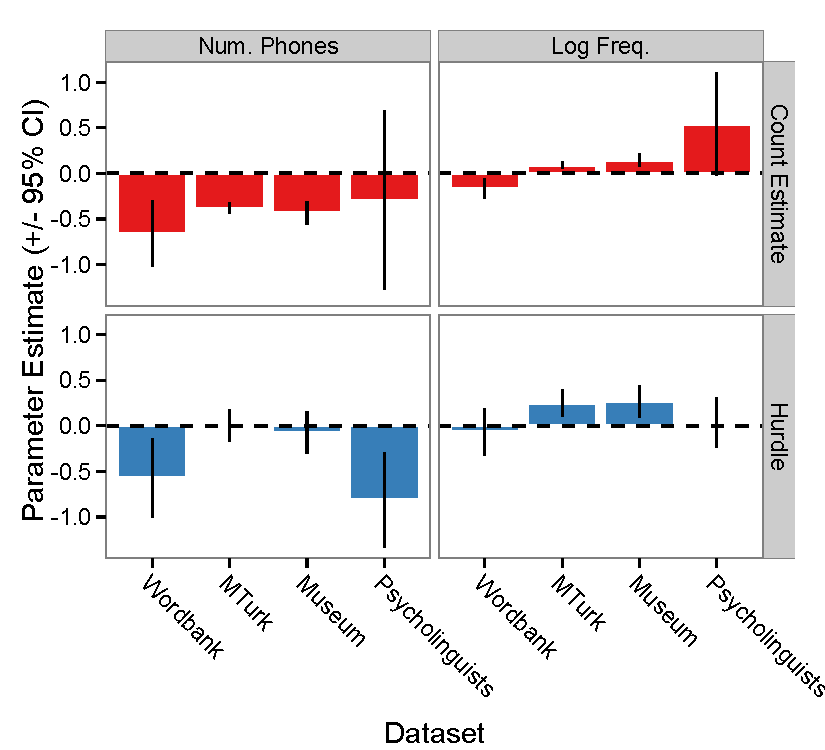
\includegraphics[width=.8\linewidth]{figures/hurdle_params.pdf}}
\caption{\label{fig:hurdles} Parameter estimates for hurdle models predicting children's first words. Models showed a high degree of consistency across datasets: first words tend to be higher frequency and have fewer phonemes. Error bars represent 95\% confidence intervals. Intercepts are omitted for clarity.}
%\vspace{-.5em}
\end{figure}

% \subsubsection{Results and Discussion}

Across datasets, input frequency and phonetic complexity consistently predicted the number of children who produced each word as their first word. As we hypothesized, in almost all cases candidate words were more likely to be first words if they were higher frequency in children's input, and if they had fewer phonemes (Figure~\ref{fig:hurdles}). In conjunction with the analyses above, these results suggest a high degree of consistency in children's first productions, independent of conceptual development, and dependent instead on linguistic input and speech production fluency.

\section{General Discussion}

What can children's first words reveal about their conceptual and linguistic development? Using parent report data, we presented three analyses, touching on the timing of productive language emergence, the distribution of conceptual categories across developmentally early and late first words, and factors that play a role in predicting which words are produced first. More than three quarters of children produced a first word prior to their first birthday, but the particular concepts these words named did not vary across age. Instead, two non-conceptual factors---input frequency and phonetic complexity---predicted the number of children who produced a particular word first.

A child's first word is a highly salient moment whose memorability to caregivers also makes it ideally suited for use in parent-report measures. Nonetheless, even when analyzed at this scale, parent report is always limited by observer bias. Although we found no evidence of retrospective biases in parents of older children over-reporting early first words, we must remain aware that there are potential issues with memory recall or other parental biases, as in any self-report measure. We dealt with these issues in several ways, including by seeking converging evidence across multiple, distinct datasets and by testing explicitly for retrospective biases. Nevertheless, the possibility of bias is present, and future studies should consider the possibility of prospective report or dense recording techniques to extend and validate our findings. 

We began by asking about the lag between comprehension and production in early language. One possible explanation for this lag is that there is a period during early infancy in which word knowledge consists of associations between auditory and visual stimuli and so there is no drive to communicate through production. In contrast to this hypothesis, our data suggest that many children are striving to communicate even quite early on. Consistent with other studies of early vocabulary \cite{tardif2007}, the productions that parents reported also included functional and communicative items---``hi,'' ``more,'' and ``no''---as well as common nouns. In sum, our work suggests that studying the very first emergence of productive speech is a rich method for adding to our understanding of language development.

\section{Acknowledgements}

Thanks to Ally Kraus for assistance with survey design and Jenni Martin and Rick Berg for help with the Museum data.

\bibliographystyle{myapacite}

\setlength{\bibleftmargin}{.125in}
\setlength{\bibindent}{-\bibleftmargin}

\bibliography{fw_cogsci}

\end{document}


